%
% Complete documentation on the extended LaTeX markup used for Insight
% documentation is available in ``Documenting Insight'', which is part
% of the standard documentation for Insight.  It may be found online
% at:
%
%     http://www.itk.org/

\documentclass{InsightArticle}


% to be able to use options in graphics
\usepackage{graphicx}
% for pseudo code
\usepackage{listings}
% subfigures
\usepackage{subfigure}

% some maths symbols
\usepackage{amstext,amssymb}

% to include accents in bliblio
\usepackage[T1]{fontenc}
\usepackage[latin1]{inputenc}

%%%%%%%%%%%%%%%%%%%%%%%%%%%%%%%%%%%%%%%%%%%%%%%%%%%%%%%%%%%%%%%%%%
%  hyperref should be the last package to be loaded.
%%%%%%%%%%%%%%%%%%%%%%%%%%%%%%%%%%%%%%%%%%%%%%%%%%%%%%%%%%%%%%%%%%
\usepackage[dvips,
bookmarks,
bookmarksopen,
backref,
colorlinks,linkcolor={blue},citecolor={blue},urlcolor={blue},
]{hyperref}

%  This is a template for Papers to the Insight Journal. 
%  It is comparable to a technical report format.

% The title should be descriptive enough for people to be able to find
% the relevant document. 
\title{Efficient N-Dimensional surface estimation using Crofton formula and run-length encoding}

% Increment the release number whenever significant changes are made.
% The author and/or editor can define 'significant' however they like.
% \release{0.00}

% At minimum, give your name and an email address.  You can include a
% snail-mail address if you like.
\author{Ga\"etan Lehmann{$^1$} {\small{and}} David Legland{$^2$}}
\authoraddress{{$^1$}INRA, UMR 1198; ENVA; CNRS, FRE 2857, Biologie du D\'eveloppement et Reproduction, Jouy en Josas, F-78350, France.\\
{$^2$}INRA, UMR 0782, G\'enie et Microbiologie des Proc\'ed\'es Alimentaire, Thiverval-Grignon, F-78850, France.}

\begin{document}
\maketitle

\ifhtml
\chapter*{Front Matter\label{front}}
\fi


\begin{abstract}
\noindent
Unlike the measure of the area in 2D or of the volume in 3D, the perimeter and the surface are not easily measurable in a discretized image.
In this article we describe a method based on the Crofton formula to measure those two parameters in a discritized image. The accuracy of
the method is discussed and tested on several known objects. An algorithm based on the run-length encoding of binary objects is presented
and compared to a brute force approach.
An implementation is provided and integrated in the LabelObject/LabelMap framework contributed earlier by the authors.
\end{abstract}

\tableofcontents

\section{Introduction}

Dans l'intro, mettre :
* mesure perimetre ou surface est important
* liste des differentes methodes pour mesures surface / perimetre
    * choix marching cubes pour comparer
* parler des facteurs de forme et introduire "roundness"
* plan de l'article

\section{Principles}
\subsection{Crofton formula}

% Crofton formula
Perimeter measure of 2D objects, surface area measure of 3D objects 
and more generally $(d-1)$-surface measure of $d$-dimensional objects 
can be expressed in a unified formalism by using the Crofton formula.
This formula consists in integrating the intercept number of the object with
lines of various orientation and positions. Its expression in
the general form is:
\begin{eqnarray}
S^{(d-1)}(X) & = & \frac{d v_d}{\pi}\int_{\mathcal{L}^d}\chi\left(X\cap L\right) dL
\end{eqnarray}
where $X$ is the structure of interest, $v_d$ is the volume of the $d$-dimensional ball,
$\mathcal{L}^d$ is the set of all lines in the $d$-dimensional space. 
The above integral is normalised such that the mass of lines hitting the unit ball 
equals $v_{d-1}$, the measure of the unit ball projection on a $(d-1)$-dimensional plane.

The Euler-Poincar\'e characteristic $\chi$ is equal to number of connected components
of the intersection of $X$ with a line $L$, or equivalently half the number of intersections
of the boundary of $X$ with the line.

% 2D and 3D
For planar and 3D cases, Equation 1 can be rewritten:
\begin{eqnarray}
P(X) & = & \pi \int_{\mathcal{L}^2} \chi \left( X \cap L \right) dL \\
S(X) & = &  4  \int_{\mathcal{L}^3} \chi \left( X \cap L \right) dL
\end{eqnarray}

\subsection{Crofton formula in discrete images}

The Crofton formula can be easily applied to discrete binary images \cite{Lang2001, Legland2007}. 
The integral over lines can be decomposed into an integral over a finite set of directions
and an integral over lines parallel to a given direction.
The number of connected components in the intersections of the structure with a discrete line
is obtained by counting the number of intercepts with its boundary.

[Ajouter une formule avec des sommes a la place des integrales]

[dire comment on calcule les poids (1) des espaces entre les droites et (2) des poids associes aux directions]
[Cas des directions principales ($d$ en $nd$) et de toutes les directions (4 en 2D et 13 en 3D)]

\subsection{Intercepts count in digital images}

The intercepts count, required to use the method described earlier, can be efficiently computed by using the run-length
encoding of the binary objects.

\subsection{Roundness}

The roundness is defined the ratio of equivalent $d$-perimeter over the measured $d$-perimeter:
\begin{eqnarray}
roundness = \frac{P_{eq}}{P}
\end{eqnarray}

Roundness takes values between $0$ and $1$. 
It is equal to $1$ for circular or spherical shapes, 
and decreases for more complicated shapes.


\section{Implementation}

The implementation of this algorithm has been done in the \verb$itk::ShapeLabelMapFilter$ class, which is already in charge of the computation of
several shape descriptors. The run-length encoding used in the \verb$itk::LabelObject$ representation is reused.
The implementation is N-dimensional and thus is usable for any image dimension. The most useful cases, 2D and 3D have been specialized
to provide a more accurate estimation by also using the diagonals -- 4 directions in 2D and 13 directions in 3D. In the 4D case and greater,
the diagonals are not used.

\subsection{N-Dimensional name}
The attribute is called {\em Perimeter} independently of the dimension of the image and is available in the \verb$itk::ShapeLabelObject$.

\subsection{Border management}

The borders of the image is considered to be in the background, so the contour of an object touching the border of the image is measured.
This was not the case in the previous (undocumented) implementation and has been proven to be misleading for many users.
It is possible to subtract the perimeter on the border to the full perimeter if the measure without the part touching the border is needed.

\subsection{Multithreading}

The architecture implemented in \verb$itk::ShapeLabelMapFilter$ use one thread per LabelObject. The perimeter estimation has been integrated in this
architecture, providing a multithreaded implementation as long as there are several LabelObjects in the input LabelMap.


The perimeter estimation is now turned on by default, but can still disabled with \verb$SetComputePerimeter(false)$ in
\verb$itk::ShapeLabelMapFilter$ if not needed. This should enhance the user experience, especially for the attributes non obviously derived
from the perimeter like the roundness.


\section{Evaluation method}

\subsection{Test shapes}

Perimeter and surface area are measured on discretization of various 2D and 3D shapes 
whose true perimeter or surface area is known.

Planar test shapes include:
\begin{itemize}
\item disks
\item ring, obtained by the difference of several disks
\item trefoil shape
\item ellipses with $a=XX$ and $b=XX$
\item rectangle with length $XX$ and width $XX$
\end{itemize}

 % Example of reconstruction of a discrete disk
\begin{figure}[!htb]
\begin{center}
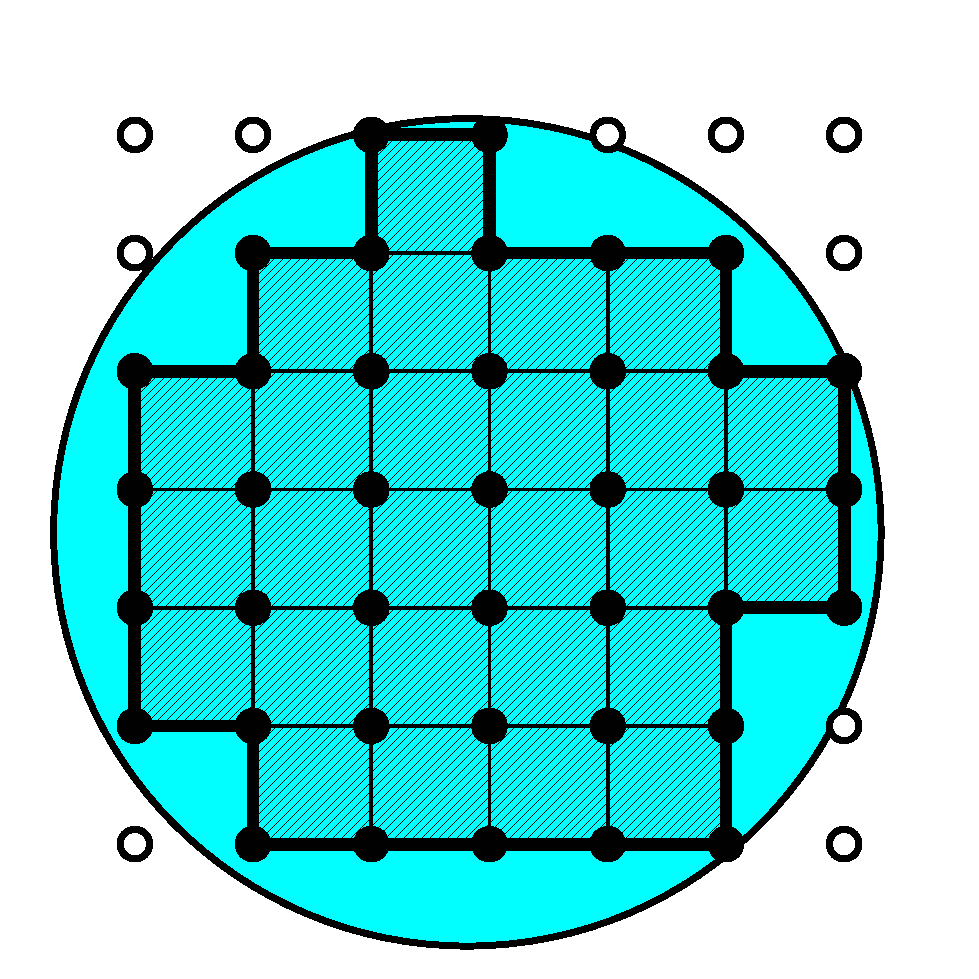
\includegraphics[width=5cm]{images/discreteDisk}
\end{center}
\end{figure}

Test shapes for 3D measurements include:
\begin{itemize}
\item balls with various radii
\item hollow ball
\item prolate and oblate ellipsoids
\item cuboids
\end{itemize}

\subsection{Shape discretization}

A 2D or 3D binary image can be considered as a subset of a rectangular grid $L_d$ where
d = 2,3. Such a grid can be written as
\begin{eqnarray}
L_d = \Delta_{1} \mathbb{Z} \times \ldots \times \Delta_{1} \mathbb{Z},
\end{eqnarray}

where the $d$-uple $(\Delta_{1},\ldots,\Delta_{d})$ defines the pixel
or voxel size. A digitization scheme represents how a continuous
structure $X$ is digitized into a binary image $X_\text{d}$. According to
the lattice scheme, $X_\text{d} = X\cap\mathbb{L}^d$. According to the
covering scheme a grid point $x$ belongs to $X_\text{d}$ if the grid
cell centered on $x$ hits $X$. 
This paper assumes isotropic resolution, i.e. $\Delta_{i}$ being the same for all $i$.

\subsection{Measurements}

For each test shape, measurements were made on
several discretisation of the shape, with various orientations and various origins.

The center of each shape was chosen at random within the center pixel or voxel of the grid.

Perimeter of 2D discretized shapes was measured using Crofton method using 2 and 4 directions, 
and by computing the length of the reconstructed contour (method ?).
Surface area of 3D discretized shapes was measured using Crofton method using 3 and 13 directions, 
and by computing the surface area of the reconstruced shape obtained by the marching cubes algorithm.
The average and the standard deviation of measurements were computed for all shapes discretized
with the same resolution. Effect of orientation was investigated by computing average and standard 
deviation of shapes having the same orientation.

\subsection{Timing evaluation}

???

\section{Accuracy}

\subsection{Global accuracy}

[Tableaux qui donnent les valeurs moyennes pour les differentes formes]

%
\begin{table}[!htb]
\begin{center}
\begin{tabular}{|c|c|c|c|} \hline 
shape		    & $U$		& $U_d^2$ & $U_d^4$		\tabularnewline \hline
disk		    & $251.33$	& $251.31$ 	& $251.32$ 	\tabularnewline
ring		    & $376.99$	& $376.99$ 	& $377.02$	\tabularnewline
rectangle  $0$ 	& $120.00$ 	&\ \ $94.24$& $112.66$	\tabularnewline
rectangle $30$  & $-$ 		& $127.23$	& $120.82$	\tabularnewline
rectangle $45$  & $-$ 		& $131.95$	& $113.18$	\tabularnewline
\hline
\end{tabular}\end{center}
\caption{\label{tab:Validate-Perimeter}
Differences between theoretical and measured perimeter of planar shapes.
Approximations were computed using $2$ and $4$ directions.
}
\end{table}

\subsection{Position effect}

[On regarde effet de la resolution et de la dispersion des mesures]
[-> 1 graphe 2D, 1 graphe 3D, avec superposition des mesures ?]

\subsection{Orientation effect}


\section{Timing}

[c'est rapide]

\section{Application}

ICOPAN


\appendix



\bibliographystyle{plain}
\bibliography{InsightJournal}
\nocite{ITKSoftwareGuide}

\end{document}

